\begin{ledgroupsized}[r]{120mm}
\footnotesize
\pstart\noindent
\textbf{Überlieferung:}
\pend
\end{ledgroupsized}
\begin{ledgroupsized}[r]{114mm}
\footnotesize
\pstart \parindent -6mm
\makebox[6mm][l]{\textit{L}}%
Konzept:
LH~XXXV~13, 3~Bl.~220\textendash221. 
Ein Bogen~2\textsuperscript{o};
Wasserzeichen		%
in Bl.~221.
Dreieinhalb Seiten.
Das Diagramm \lbrack\textit{Fig.~9}\rbrack\ wird, trotz seiner Platzierung auf Bl. 221~r\textsuperscript{o}, als zu Bl.~220~v\textsuperscript{o} und dem Text von Art.~(14) zugehörig gedeutet und am entsprechenden Ort wiedergegeben (S.~\pageref{Fig:LH_35_13_03_220-221_d9_221r}). 
\pend
\end{ledgroupsized}
\selectlanguage{latin}
\vspace{8mm}
\pstart\noindent%
\edlabel{35_13_03_220-221_9a}%
\edtext{}{%
\xxref%
{35_13_03_220-221_9a}{35_13_03_220-221_9b}%
\lemma{\href{\Scan{LH_35_13_03_220r}}{\lbrack220~r\textsuperscript{o}\rbrack}}%
\Bfootnote{%
\textit{(1)}~Si globus in globum oblique incurrat %
\textit{(a)}~non ideo minus tamen %
\textit{(b)}~sed tamen centrice, nulla %
\textit{(aa)}~est %
\textit{(bb)}~oritur circulatio. Centrice autem fit concursus si %
\textit{(aaa)}~li %
\textit{(bbb)}~recta perpendicularis %
\textit{(2)}~Concursus %
\textit{(a)}~corporum %
\textit{(b)}~corporis intelligitur factus in recta. %
\textit{(3)}~(1) Omne %
\textit{(a)}~ictu %
\textit{(b)}~corpus %
\textit{(aa)}~videtur percursum\lbrack\textit{!}\rbrack\ %
\textit{(bb)}~cen %
\textit{(cc)}~percutitur~\textit{L}}}%
\href{\Scan{LH_35_13_03_220r}}{\lbrack220~r\textsuperscript{o}\rbrack}
\pend
\begin{edfigure}[0em][0.7em]    	%
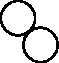
\includegraphics[scale=1]{gesamttex/edit_VIII-4/images/LH_35_13_03_220-221_d1_220r.pdf}
\edcaption[0.25em]{\lbrack\textit{Fig.~1}\rbrack}
\end{edfigure}
\pstart\noindent
(1) Omne corpus percutitur\edlabel{35_13_03_220-221_9b}
in recta perpendiculari ad superficiem\indexS{recta perpendicularis ad superficiem} percussi 
in puncto contactus.\indexS{punctum contactus}
\pend
\pstart
(2) Hinc si plura sint puncta\indexS{punctum contactus}
\edtext{contactus\lbrack,\rbrack\ percussum}{%
\lemma{contactus}%
\Bfootnote{%
\textit{(1)}~percursum %
\textit{(2)}~percussum~\textit{L}}}
est in pluribus rectis 
\edtext{simul, et perinde}{%
\lemma{simul,}%
\Bfootnote{%
\textit{(1)}~perinde %
\textit{(2)}~et perinde~\textit{L}}}
est ac si simul a pluribus corporibus fuisset 
\edlabel{35_13_03_220-221_1a}%
\edtext{}{\xxref{35_13_03_220-221_1a}{35_13_03_220-221_1b}%
\lemma{percussum}%
\Bfootnote{%
\textit{(1)}~\bars{Et quia \textit{erg.}} fieri potest ut eadem recta non sit perpendicularis ad utriusque concurrentium %
\textit{(2)}~(3) Fieri~\textit{L}}}%
percussum.
\pend
\begin{edfigure}[1em][1em]    	%
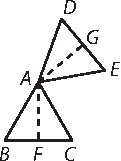
\includegraphics[scale=1]{gesamttex/edit_VIII-4/images/LH_35_13_03_220-221_d2_220r.pdf}
\edcaption{\edtext{\lbrack\textit{Fig.~2}\rbrack}{%
\lemma{\lbrack\textit{Fig.~2}\rbrack}%
\Cfootnote[nonum]{%
Ein gestrichener Entwurf zum Diagramm wird nicht wiedergegeben.}}}
\end{edfigure}
\pstart
(3) Fieri\edlabel{35_13_03_220-221_1b}
aliquando potest ut plures sint perpendiculares ad superficiem\indexS{perpendicularis ad superficiem} 
in puncto contactus,\indexS{punctum contactus}
sed tunc eligenda est perpendicularis\indexS{perpendicularis primaria}
\edtext{primaria. Et hoc fit}{%
\lemma{primaria.}%
\Bfootnote{%
\textit{(1)}~Hinc %
\textit{(a)}~f %
\textit{(b)}~fier %
\textit{(c)}~fieri %
\textit{(d)}~fieri potest, ut %
\textit{(2)}~Et hoc fit~\textit{L}}}
\edtext{cum angulus quasi quidam}{%
\lemma{cum}%
\Bfootnote{%
\textit{(1)}~angulum quasi quendam %
\textit{(2)}~angulus quasi quidam~\textit{L}}} 
est in superficie corporis, ut in vertice pyramidis.\indexS{pyramis}\indexS{vertex pyramidis} 
Hinc si duae pyramides\indexS{pyramis} \textit{ABC} et \textit{ADE} concurrant in
\edtext{puncto \textit{A}, fiet}{%
\lemma{puncto \textit{A},}%
\Bfootnote{%
\textit{(1)}~vir %
\textit{(2)}~fiet~\textit{L}}} 
\edtext{percu\lbrack s\rbrack sio\indexS{percussio}}{%
\lemma{}%
\Bfootnote{%
percursio %
\textit{L ändert Hrsg.}}}
ipsius \textit{ABC} in \textit{AF}, et ipsius \textit{ADE} in \textit{AG}, licet rectae \textit{AF} et \textit{AG} non sint in directum, quod tamen fieret, si essent globi.\indexS{globus}
\pend
\begin{edfigure}[1em][1em]    	%
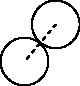
\includegraphics[scale=1]{gesamttex/edit_VIII-4/images/LH_35_13_03_220-221_d3_220r.pdf}
\edcaption[0.25em]{\lbrack\textit{Fig.~3, gestr.}\rbrack}
\end{edfigure}
\pstart
\edtext{(4)}{%
\lemma{}%
\Bfootnote{(4) \textit{erg.~L}}} 
Et ita patet fieri posse ut duo corpora concurrentia\indexS{corpora concurrentia} 
diversas accipiant directiones\indexS{directio} seu lineas percussionis;\indexS{linea percussionis}
quod impossibile est in
\edtext{corporibus, quae}{%
\lemma{corporibus,}%
\Bfootnote{%
\textit{(1)}~quae unum tantum habeant %
\textit{(2)}~quae~\textit{L}}} 
unum tantum habent planum
\edtext{tangens\indexS{planum tangens} in}{%
\lemma{tangens}%
\Bfootnote{%
\textit{(1)}~in punctis %
\textit{(2)}~in~\textit{L}}} 
quocunque puncto superficiei, adeoque et in puncto
\edtext{concursu\lbrack s\rbrack;\indexS{punctum concursus}}{%
\lemma{}%
\Bfootnote{concursu \textit{L ändert Hrsg.}}} 
quo posito oportet planum tangens\indexS{planum tangens} esse duobus corporibus commune. 
\pend
\begin{edfigure}[1em][1em]    	%
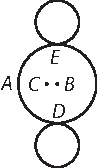
\includegraphics[scale=1]{gesamttex/edit_VIII-4/images/LH_35_13_03_220-221_d4_220r.pdf}
\edcaption{\edtext{\lbrack\textit{Fig.~4}\rbrack}{%
\lemma{\lbrack\textit{Fig.~4}\rbrack}%
\Cfootnote[nonum]{%
Ein gestrichener Entwurf zum Diagramm wird nicht wiedergegeben.}}}
\end{edfigure}
\pstart
(5) Si recta percussionis,\indexS{recta percussionis} transeat per centrum gravitatis\indexS{centrum gravitatis}
\edtext{corporis, percussio}{%
\lemma{corporis,}%
\Bfootnote{%
\textit{(1)}~linea %
\textit{(2)}~percussio~\textit{L}}} 
est centrica,\indexS{percussio centrica} sin minus eccentrica.\indexS{percussio eccentrica} Ut si in sphaera
\edtext{\textit{A}}{%
\lemma{}%
\Bfootnote{\textit{A} \textit{erg.~L}}} 
(ob materiae heterogeneitatem) non coincidant centrum sphaerae
\edtext{\textit{B}}{%
\lemma{}%
\Bfootnote{\textit{B} \textit{erg.~L}}} 
et centrum gravitatis\indexS{centrum gravitatis} \textit{C},
\edtext{eaque percutiatur}{%
\lemma{eaque}%
\Bfootnote{%
\textit{(1)}~ab alia %
\textit{(2)}~percutiatur~\textit{L}}} 
ab alio corpore quocunque, et
\edtext{utcunque, in}{%
\lemma{utcunque,}%
\Bfootnote{%
\textit{(1)}~percussio \bars{erit \textit{streicht Hrsg.}} %
\textit{(a)}~eccentrica %
\textit{(b)}~in linea quae %
\textit{(2)}~in~\textit{L}}} 
puncto \textit{D}, quod non cadat in rectam \textit{BC}, 
\edtext{percussio erit}{%
\lemma{percussio}%
\Bfootnote{%
\textit{(1)}~In omni %
\textit{(2)}~erit~\textit{L}}}
eccentrica.\indexS{percussio eccentrica}
\pend
\pstart
(6) In omni percussione eccentrica\indexS{percussio eccentrica}
\edtext{oritur gyratio\indexS{gyratio}}{%
\lemma{oritur}%
\Bfootnote{%
\textit{(1)}~(\protect\vphantom)si nihil imped %
\textit{(2)}~gyratio~\textit{L}}} 
percussi circa centrum,\indexS{centrum gravitatis} nisi forte sit quod impediat.
Velut si sphaera \textit{A} percutiatur simul in \textit{D} et \textit{E}, eccentrice,\indexS{sphaera percussa eccentrice}
sed \textit{CBE} et \textit{CBD} sint anguli aequales, 
patet compensationem gyrationis\indexS{gyratio}\indexS{compensatio gyrationis} utrinque fieri, adeoque gyrationem\indexS{gyratio}
\edlabel{35_13_03_220-221_2a}%
\edtext{}{\xxref{35_13_03_220-221_2a}{35_13_03_220-221_2b}%
\lemma{cessare}%
\Bfootnote{%
\textit{(1)}~Non %
\textit{(2)}~(7) Nulla~\textit{L}}}%
cessare. 
\pend
\begin{edfigure}[1em][1em]     %
\hfill
\includegraphics[scale=1]{%
gesamttex/edit_VIII-4/images/LH_35_13_03_220-221_d5_220r.pdf%
}%
\hfill
\protect\raisebox{.5ex}{%
\includegraphics[scale=1]{%
gesamttex/edit_VIII-4/images/LH_35_13_03_220-221_d6_220r.pdf}}%
\hfill%
\protect\raisebox{2.25ex}{%
\includegraphics[scale=1]{%
gesamttex/edit_VIII-4/images/LH_35_13_03_220-221_d7_220r.pdf}}
\hfill
\edcaption{%
\hspace*{10mm}
\lbrack\textit{Fig.~5}\rbrack \hspace*{20mm}
\lbrack\textit{Fig.~6, gestr.}\rbrack \hspace*{15mm}
\lbrack\textit{Fig.~7, gestr.}\rbrack
}
\end{edfigure}
\pstart 
(7) Nulla\edlabel{35_13_03_220-221_2b}
autem fiet gyratio\indexS{gyratio} si percussio sit centrica.\indexS{percussio centrica} Hinc 
\edtext{si sphaerae sint homogenea\lbrack e\rbrack, fieri}{%
\lemma{si}%
\Bfootnote{%
\textit{(1)}~sphaera sit homogenea %
\textit{(2)}~sphaerae sint \bars{homogenea \textit{ändert Hrsg.}} , fieri~\textit{L}}}
non potest,
\edtext{ut sphaeris inter se concurrentibus\indexS{sphaerae concurrentes} neque}{%
\lemma{ut}%
\Bfootnote{%
\textit{(1)}~duae sphae %
\textit{(2)}~sphaeris \bars{solis \textit{erg.~u. gestr.}} inter se concurrentibus
\textit{(a)}~oriatur gyratio,
\textit{(aa)}~secus foret %
\textit{(bb)}~nisi
\textit{(b)}~neque~\textit{L}}} 
alio obstaculo existente, oriatur gyratio;\indexS{gyratio} secus
est si quid adsit, quod sphaerae procursum secundum directionem
\edtext{receptam}{%
\lemma{}%
\Bfootnote{receptam \textit{erg.~L}}} 
quoad partem impediat, ut si sphaera \textit{A} inveniat obstaculum \textit{B}\lbrack:\rbrack\ tunc enim progredietur cum gyratione.\indexS{gyratio}
\pend
\pstart
\edlabel{35_13_03_220-221_12a}%
\edtext{(8) Ex}{%
\lemma{(8)}%
\Bfootnote{%
\textit{(1)}~Si %
\textit{(2)}~Hactenus %
\textit{(3)}~Ex~\textit{L}}} 
his regulis accedente conservatione\indexS{conservatio potentiae}
\edtext{potentiae, tam}{%
\lemma{potentiae,}%
\Bfootnote{%
\textit{(1)}~et %
\textit{(2)}~tam~\textit{L}}} 
absolutae\indexS{potentia absoluta}\indexS{conservatio potentiae absolutae} quam
\edtext{respectivae\lbrack,\rbrack\indexS{potentia respectiva}\indexS{conservatio potentiae respectivae} possunt derivari}{%
\lemma{respectivae}%
\Bfootnote{%
\textit{(1)}~oritur %
\textit{(2)}~possunt derivari~\textit{L}}} 
phaenomena concurrentium\indexS{phaenomena concurrentium} duarum sphaerarum homogenearum.
\pend
\pstart
Veniamus jam ad concursum trium corporum,\indexS{concursus trium corporum} 
quae materia adhuc intacta est,
sed stabiliamus 
\edtext{primum regulas}{%
\lemma{primum}%
\Bfootnote{%
\bars{\textit{(1)}~haec %
\textit{(2)}~has \textit{gestr.}}
regulas~\textit{L}}}
per quas
solvi possint casus omnes. Et primum quidem pro certo sumo conservari\indexS{conservatio potentiae absolutae} semper eandem potentiam absolutam.\indexS{potentia absoluta}
\pend 
\begin{edfigure}[1em][1em]    	%
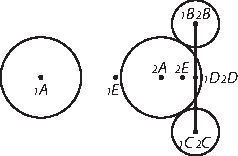
\includegraphics[scale=1]{gesamttex/edit_VIII-4/images/LH_35_13_03_220-221_d8_220r.pdf}
\edcaption{\lbrack\textit{Fig.~8, gestr.}\rbrack}
\end{edfigure}
\pstart 
(9) Deinde assumo quoque semper conservari eandem potentiam progressus,\indexS{progressus}\indexS{potentia progressus}\indexS{conservatio potentiae progressus}
\edtext{adeoque centrum}{%
\lemma{adeoque}%
\Bfootnote{%
\textit{(1)}~celeritatem %
\textit{(2)}~centrum~\textit{L}}} 
gravitatis\indexS{centrum gravitatis totale concurrentium}
\edtext{totale concurrentium}{%
\lemma{}%
\Bfootnote{totale concurrentium \textit{erg.~L}}} 
semper progredi in eadem recta eademque celeritate.\indexS{progressus centri gravitatis totalis in eadem recta eademque celeritate} %
\pend
\pstart
(10) Assumo etiam semper conservari eandem 
potentiam respectivam\indexS{potentia respectiva}\indexS{conservatio potentiae respectivae} 
quae consistit in recessu unius corporis ab alio,\indexS{recessus unius corporis ab alio} 
vel in circulatione\indexS{circulatio} qua saltem a se invicem recedere\indexS{recessus corporum a se invicem} conantur.%
\edlabel{35_13_03_220-221_12b}
\pend
\pstart
\indent (11) Hinc ubi abest circulatio\indexS{circulatio}
\edtext{(ut in concursu sphaerarum)}{%
\lemma{}%
\Bfootnote{(ut in concursu sphaerarum) \textit{erg.~L}}} 
necesse est potentiam respectivam\indexS{potentia respectiva} 
\edtext{spectari in solo}{%
\lemma{spectari}%
\Bfootnote{%
\textit{(1)}~in solo r %
\textit{(2)}~in sola %
\textit{(a)}~in solo~\textit{L}}}
a se invicem recessu.\indexS{recessus corporum a se invicem}
\pend
\pstart
(12) Si plura sint corpora potentia
\edtext{respectiva totalis\indexS{potentia respectiva totalis} componetur 
ex potentia respectiva recessus centri unius cujusque a centro gravitatis reliquorum\indexS{centrum gravitatis reliquorum corporum}\indexS{potentia respectiva recessus a centro} et}{%
\lemma{respectiva}%
\Bfootnote{%
\textit{(1)}~spectabitur in %
\textit{(2)}~totalis \lbrack...\rbrack\  recessus %
\bars{\textit{(1)}~centro \textit{(2)}~centri \textit{erg.}} %
unius \lbrack...\rbrack\  reliquorum %
\textit{(a)}~qua ostendi semper eandem potentiam respectivam prodire. Nam %
\textit{(aa)}~unum %
\textit{(bb)}~duo %
\textit{(b)}~quaecunque simul sumta pr %
\textit{(c)}~et~\textit{L}}} 
potentia respectiva\indexS{potentia respectiva} reliquorum inter se.
\edtext{Qua ratione idem provenire ostensum est, utcunque fiat combinatio.\indexS{combinatio}}{%
\lemma{Qua \lbrack...\rbrack\ combinatio}%
\Cfootnote{%
Siehe bspw. das Konzept N.\;\ref{58300}.}}
\pend
\pstart
\href{\Scan{LH_35_13_03_220v}}{\lbrack220~v\textsuperscript{o}\rbrack}\
(13) Veniamus jam
\edtext{ad concursum}{%
\lemma{ad}%
\Bfootnote{%
\textit{(1)}~casum %
\textit{(2)}~concursum~\textit{L}}} 
trium sphaerarum,\indexS{concursus trium sphaerarum} quas ponamus esse
\edtext{homogeneas\indexS{sphaerae homogeneae} ut concursus sit centricus,\indexS{concursus centricus}}{%
\lemma{homogeneas}%
\Bfootnote{%
\textit{(1)}~et duras, ut concursus %
\textit{(2)}~ut concursus sit %
\textit{(a)}~eccentricus %
\textit{(b)}~centricus,~\textit{L}}} 
et duras,\indexS{sphaerae durae} ne pars virium\indexS{vis} in exiguis partibus intereat. 
Et ut a facilioribus incipiamus, ponamus duas
\edtext{esse quiescentes,}{%
\lemma{esse}%
\Bfootnote{%
\textit{(1)}~aequales inter se %
\textit{(2)}~quiescentes,~\textit{L}}}
et aequales inter se,\indexS{spherae quiescentes aequales} 
et eodem modo se habentes ad tertiam ejusve motum.\indexS{motus}
\pend
\begin{edfigure}[0.75em][1em]    	%
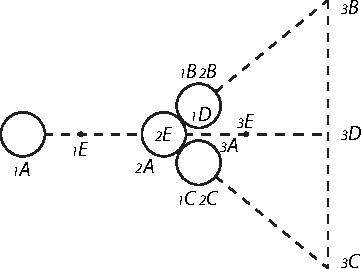
\includegraphics[scale=1]{gesamttex/edit_VIII-4/images/LH_35_13_03_220-221_d9_221r.pdf}
\edcaption[0pt]{%
\edtext{\lbrack\textit{Fig.~9 (Bl.~\href{\Scan{LH_35_13_03_221r}}{221~r\textsuperscript{o}})}\rbrack}{%
\lemma{\lbrack\textit{Fig.~9}\rbrack}%
\Cfootnote[nonum]{%
Leibniz hat das Diagramm auf Bl.~221~r\textsuperscript{o} gezeichnet.
Dass dies allerdings wohl nur aus Platzgründen geschehen ist, und die Figur zum Text auf Bl.~220~v\textsuperscript{o} gehört, legen folgende Umstände nahe:
Sie befindet sich in Falznähe, direkt gegenüber Art.~(14); 
sie wird in sämtlichen Ausführungen und Berechnungen der folgenden Artikel vorausgesetzt; 
bereits auf Bl.~220~r\textsuperscript{o}, unmittelbar nach Art.~(8), hatte Leibniz zu einer ähnlichen Zeichnung angesetzt (siehe die gestrichene Vorstufe \lbrack\textit{Fig.~8}\rbrack). 
Aus den genannten Gründen wird das Diagramm an dieser Stelle wiedergegeben.}}%
}
\pagelabel{Fig:LH_35_13_03_220-221_d9_221r}
\end{edfigure}
\pstart
\edtext{(14) Sit}{%
\lemma{(14)}%
\Bfootnote{%
\textit{(1)}~Sint %
\textit{(2)}~Sit~\textit{L}}} 
globus\indexS{globus} in motu
\edtext{cujus centrum\indexS{centrum gravitatis}}{%
\lemma{}%
\Bfootnote{cujus centrum \textit{erg.~L}}} 
\textit{A}, globi
\edtext{aequales}{%
\lemma{}%
\Bfootnote{aequales \textit{erg.~L}}} 
quiescentes\indexS{globi aequales quiescentes}
\edtext{quorum centra\indexS{centrum gravitatis}}{%
\lemma{}%
\Bfootnote{quorum centra \textit{erg.~L}}} 
\textit{B} et \textit{C}; centrum
commune\indexS{centrum gravitatis commune} ipsorum \textit{B} et \textit{C} sit \textit{D}, 
et centrum commune omnium\indexS{centrum gravitatis commune omnium} \textit{E}, 
\edtext{erit \lbrack\textit{CD}\rbrack\ aequal.}{%
\lemma{}%
\Bfootnote{%
erit
\bars{\textit{BC} \textit{ändert Hrsg.}}
aequal.~\textit{L}}} 
\textit{BD}
et \textit{AE}
\edtext{erit ad \textit{B}\lbrack\textit{D}\rbrack, ut glob.~\textit{C} $+$ glob.~\lbrack\textit{B}\rbrack\ ad}{%
\lemma{}%
\Bfootnote{%
erit ad 
\bars{\textit{BE} \textit{ändert Hrsg.}} %
ut glob. \textit{C} $+$ glob.
\bars{\textit{D} \textit{ändert Hrsg.}} %
ad~\textit{L}}}
glob. \textit{A}. Situs primus erit \textit{\ind{1}A}, \textit{\ind{1}B}, \textit{\ind{1}C}, \textit{\ind{1}D}, \textit{\ind{1}E}; situs secundus ipse scilicet 
situs concursus\indexS{concursus} 
erit \textit{\ind{2}A}, \textit{\ind{2}B}, \textit{\ind{2}C}, \textit{\ind{2}D}, \textit{\ind{2}E}, ubi ob
\edtext{quietem corporum}{%
\lemma{quietem}%
\Bfootnote{%
\textit{(1)}~punctorum %
\textit{(2)}~corporum~\textit{L}}} 
\textit{B} et \textit{C} adeoque et puncti \textit{D}, coincident \textit{\ind{1}B}, \textit{\ind{1}C}, \textit{\ind{1}D}, cum ipsis \textit{\ind{2}B}, \textit{\ind{2}C}, \textit{\ind{2}D}. 
Situs tertius erit qui designabit celeritatem post concursum,\indexS{concursus} 
\edtext{ita ut tantum}{%
\lemma{ita ut}%
\Bfootnote{%
\textit{(1)}~tam ut %
\textit{(2)}~tantum~\textit{L}}}
temporis intersit inter situm secundum, et situm tertium \textit{\ind{3}A}, \textit{\ind{3}B}, \textit{\ind{3}C}, \textit{\ind{3}D}, \textit{\ind{3}E}, quantum temporis interfuit inter situm primum et secundum. Quaeritur modus determinandi situm tertium, ex primo, et secundo. 
\pend
\pstart
(15) Et quidem ante omnia datur punctum \textit{\ind{3}E}, per artic. 9.
\edtext{Nam debet}{%
\lemma{Nam}%
\Bfootnote{%
\textit{(1)}~quia \textit{\ind{2}E\ind{3}E} aequ. \textit{\ind{1}E\ind{2}E}, %
\textit{(2)}~debet~\textit{L}}} 
tantum in recta \textit{\ind{1}E\ind{2}E} continuata sumi punctum \textit{\ind{3}E}, sic, ut sit recta
\edtext{\textit{\ind{2}E\ind{3}E} aequalis}{%
\lemma{}%
\Bfootnote{\textit{\ind{2}E\ind{3}E} \bars{sit \textit{streicht Hrsg.}} aequalis~\textit{L}}} 
ipsi \textit{\ind{1}E\ind{2}E}.
\pend
\pstart
(16) Si jam
\edtext{corpora \textit{B}, et \textit{C} per}{%
\lemma{corpora}%
\Bfootnote{%
\textit{(1)}~\textit{B} et \textit{C} no %
\textit{(2)}~\textit{B}, et \textit{C} per~\textit{L}}} 
ictum\indexS{ictus} non recederent inter se, 
omnis potentia respectiva\indexS{potentia respectiva} maneret in solo recessu\indexS{recessus} ipsius \textit{A} ab ipso \textit{D}, seu foret \textit{\ind{3}A\ind{3}D} aequalis ipsi
\edtext{\textit{\ind{1}A\ind{1}D}. Sed \textit{B} et \textit{C} a se invicem recedere\indexS{recessus corporum a se invicem} debent,}{%
\lemma{\textit{\ind{1}A\ind{1}D}.}%
\Bfootnote{%
\textit{(1)}~Sed quia \textit{B} et \textit{C} a se recedere necesse est %
\textit{(2)}~Sed \textit{B} \lbrack...\rbrack\  recedere debent,~\textit{L}}}
ut mox ostendam
\edtext{(artic.~17).}{%
\lemma{}%
\Bfootnote{(artic.~17) \textit{erg.~L}}}
Ergo fit \textit{\ind{3}A\ind{3}D} minor ipsa \textit{\ind{1}A\ind{1}D}. 
\pend
\pstart
(17)
\edtext{Nimirum per}{%
\lemma{Nimirum}%
\Bfootnote{%
\textit{(1)}~ex %
\textit{(2)}~quia nulla fit %
\textit{(3)}~oportet %
\textit{(4)}~per~\textit{L}}} 
artic.~1. oportet \textit{\ind{3}B} esse in recta \textit{\ind{2}A\ind{2}B}, et \textit{\ind{3}C} in recta \textit{\ind{2}A\ind{2}C} ergo \textit{\ind{3}B\ind{3}C} est major quam \textit{\ind{2}B\ind{2}C},
\edtext{seu \textit{B} et \textit{C}}{%
\lemma{seu}%
\Bfootnote{%
\textit{(1)}~recedunt
\textit{(2)}~int %
\textit{(3)}~\textit{B} et \textit{C}~\textit{L}}} 
a se invicem recedunt.\indexS{recessus corporum a se invicem}
\pend
\pstart
(18) Est autem
\edtext{recta \textit{\ind{3}B\ind{3}C}}{%
\lemma{recta}%
\Bfootnote{%
\textit{(1)}~\textit{\ind{3}A\ind{3}C} %
\textit{(2)}~\textit{\ind{3}B\ind{3}C}~\textit{L}}} 
normalis ad ipsam \textit{AD}, 
\edtext{et \textit{\ind{3}A\ind{3}\textup{\lbrack}C\textup{\rbrack}} aequalis ipsi \textit{\ind{3}B\ind{3}\textup{\lbrack}A\textup{\rbrack}}, quoniam}{%
\lemma{}%
\Bfootnote{%
et 
\bars{\textit{\ind{3}A\ind{3}D} \textit{ändert Hrsg.}}
aequalis ipsi 
\bars{\textit{\ind{3}B\ind{3}D} \textit{ändert Hrsg.}} ,
quoniam~\textit{L}}}
scilicet ante concursum\indexS{concursus} eodem modo se habet \textit{A} ad \textit{B} et \textit{C}, ergo et post
\edtext{concursum.\indexS{concursus} Ideo superest}{%
\lemma{concursum}%
\Bfootnote{%
\textit{(1)}~Superest nunc %
\textit{(2)}~Ideo superest~\textit{L}}} 
ut definiamus punctum \textit{\ind{3}D}. Hoc enim dato,
necesse est etiam dari puncta \textit{\ind{3}B} et \textit{\ind{3}C} quoniam per \textit{\ind{3}D} ducendo normalem ad \textit{AD}, secabit ea rectas \textit{\ind{2}A\ind{2}B} et \textit{\ind{2}A\ind{2}C} in punctis \textit{\ind{3}B} 
\edlabel{35_13_03_220-221_3a}%
\edtext{}{\xxref{35_13_03_220-221_3a}{35_13_03_220-221_3b}%
\lemma{et \textit{\ind{3}C}.}%
\Bfootnote{%
\textit{(1)}~(19) Itaque jam ad calculum quendam veniendum erit. %
\textit{(a)}~\textit{\ind{1}A\ind{1}D} vocetur %
\textit{(b)}~\textit{\ind{1}E\ind{1}D} vocetur \textit{a}. %
\textit{(aa)}~\textit{\ind{1}A\ind{1}E} er %
\textit{(bb)}~\textit{\ind{1}E\ind{1}A} repraesentabitur per $b+c$. Est enim \textit{\ind{1}E\ind{1}D} ad \textit{\ind{1}E\ind{1}A}, ut \textit{a} ad %
\textit{(aaa)}~$a+b$ %
\textit{(bbb)}~$b+c$, posito \textit{a} repraesentare magnitudinem globi, et \textit{b}, \textit{c}, 
\textit{(aaaa)}~glo
\textit{(bbbb)}~magnitudinem globorum \textit{B} et \textit{C}. Et %
\textit{(aaaaa)}~\textit{\ind{1}A} %
\textit{(bbbbb)}~\textit{\ind{1}D\ind{1}B} vel \textit{\ind{1}D\ind{1}C} esto \textit{d} %
\textit{(aaaaa-a)}~. Potentia ante ictum erit %
\textit{(bbbbb-b)}~et \textit{\ind{1}A\ind{1}D} erit
$\ind{1}A\ind{1}E+\ind{1}E\ind{1}D$ seu %
\textit{(aaaaa-aa)}~erit %
\textit{(bbbbb-bb)}~\textit{\ind{1}A\ind{1}D} erit $a+b+c$ %
\textit{(2)}~(19) Itaque~\textit{L}}}%
et \textit{\ind{3}C}.
\pend
\pstart
(19) Itaque\edlabel{35_13_03_220-221_3b}
jam ad calculum quendam veniendum erit. 
Concursus\indexS{concursus} repraesentatur per triangulum \textit{\ind{2}A\ind{2}B\ind{2}C}\lbrack,\rbrack\ tangat autem \textit{A} ipsum \textit{B} in \textit{F}, et ipsum \textit{C}
\edtext{in \textit{G}. Patet \textit{AF}}{%
\lemma{in \textit{G}.}%
\Bfootnote{%
\textit{(1)}~Fiet recta %
\textit{(2)}~Patet %
\textit{(a)}~rectam \textit{AFB} %
\textit{(b)}~\textit{AF}~\textit{L}}}
et \textit{AG} esse aequales, cum sint radius globi\indexS{globus} \textit{A}, sed \textit{BF} esse radium globi \textit{B} et \textit{CG} radium globi \textit{C}, 
\edtext{adeoque globi\indexS{globus} repraesentabuntur per harum rectarum sive radiorum cubos, eruntque}{%
\lemma{adeoque}%
\Bfootnote{%
\textit{(1)}~globos repraesentabimus %
\textit{(2)}~globi repraesentabuntur per %
\textit{(a)}~has rectas seu per radios %
\textit{(b)}~harum rectarum sive radiorum cubos, %
\textit{(aa)}~erit %
\textit{(bb)}~eruntque~\textit{L}}}
\textit{a}, \textit{b}, \textit{c}, ut cubi ipsarum \textit{AF}, \textit{BF}, 
\edtext{\lbrack\textit{C}\rbrack\textit{G}.}{%
\lemma{}%
\Bfootnote{%
\textit{BG} %
\textit{L ändert Hrsg.}}}
Si pro globis\indexS{globus} adhibeamus cylindros\indexS{cylinder} aequalium altitudinum, erunt corpora, ipsi nempe cylindri, ut radiorum
\edlabel{35_13_03_220-221_10a}%
\edtext{}{%
\xxref%
{35_13_03_220-221_10a}{35_13_03_220-221_10b}%
\lemma{quadrata.}%
\Bfootnote{%
\textit{(1)}~Sit
\textit{(2)}~Jam %
\textit{(3)}~Porro %
\textit{(4)}~(20) %
\textit{(a)}~Sit %
\textit{(b)}~\textit{\ind{1}A\ind{1}E} ad \textit{\ind{1}A\ind{1}D}  ut %
\textit{(c)}~\textit{\ind{1}A\ind{1}D}, \textit{\ind{1}A} %
\textit{(d)}~\textit{\ind{1}A\ind{1}D},~\textit{L}}}%
quadrata. 
\pend
\pstart
(20) \textit{\ind{1}A\ind{1}D},\edlabel{35_13_03_220-221_10b}
\textit{\ind{1}A\ind{1}E}, \textit{\ind{1}D\ind{1}E} ut $a+b+c$, $b+c$, \textit{a}. 
\pend
\pstart
(21) \textit{\ind{2}D\ind{2}A}, sic investigatur\lbrack:\rbrack\ 
trianguli \textit{\ind{2}A\ind{2}B\ind{2}C} datur basis \textit{\ind{2}B\ind{2}C},
\edtext{seu bis \textit{\ind{2}D\ind{2}B},}{%
\lemma{}%
\Bfootnote{seu bis \textit{\ind{2}D\ind{2}B} \textit{erg.~L}}}
dantur latera duo inter se aequalia $AF+BF$, et \textit{\ind{2}A\ind{2}D} erit altitudo, 
quae habetur si a quadrato ipsius $AF+BF$, detrahatur quadratum ipsius \textit{\ind{2}D\ind{2}B} 
fietque $\surd\llcorner\;AF^2+BF^2+2AF\cdot BF-\ind{2}B\ind{2}D^2\lrcorner=$
\edtext{\textit{\ind{2}A\ind{2}D}. Et praeterea}{%
\lemma{\textit{\ind{2}A\ind{2}D}.}%
\Bfootnote{%
\textit{(1)}~Et fiet %
\textit{(2)}~Et praeterea %
\textit{(a)}~erit %
\textit{(b)}~ut~\textit{L}}} 
ut in 20, ita hic erit \textit{\ind{2}A\ind{2}D}, \textit{\ind{2}A\ind{2}E}, 
\textit{\ind{2}D\ind{2}E} ut $a+b+c$,
\edlabel{35_13_03_220-221_4a}%
\edtext{}{%
{\xxref%
{35_13_03_220-221_4a}{35_13_03_220-221_4b}}%
\lemma{$b+c$, \textit{a}.}%
\Bfootnote{%
\textit{(1)}~et %
\textit{(2)}~(21) %
\textit{(3)}~(22) Et~\textit{L}}}%
$b+c$, \textit{a}.
\pend
\pstart
(22) Et%
\edlabel{35_13_03_220-221_4b}
fiet $\ind{1}E\ind{2}E=\ind{1}E\ind{1}D-\ind{2}D\ind{2}E=\overline{a:\overline{a+b+c}}$, $\overline{\ind{1}A\ind{1}D-\ind{2}A\ind{2}D}$.
\pend
\pstart
\edtext{(23) Celeritas mobilis \textit{A} est}{%
\lemma{(23)}%
\Bfootnote{%
\textit{(1)}~Potentia ante ictum erat %
\textit{(a)}~\textit{\ind{1}A} %
\textit{(b)}~\textit{a} %
\textit{(2)}~Celeritas mobilis \textit{A} %
\textit{(a)}~\textit{\ind{1}A} %
\textit{(b)}~est~\textit{L}}} 
$\ind{1}A\ind{2}A=\ind{1}A\ind{1}D-
\edtext{\ind{2}D\ind{2}A$. Ergo erit \textit{\ind{1}A\ind{2}A}}{%
\lemma{\textit{\ind{2}D\ind{2}A}.}%
\Bfootnote{%
\textit{(1)}~Ergo ejus potentia ducta in %
\textit{(2)}~erit \textit{a} in $\protect\fbox{2}\, \ind{1}A\ind{1}D-\ind{2}D\ind{2}A$ %
\textit{(3)}~Ergo erit %
\textit{(a)}~\textit{\ind{1}A\ind{2}A} ad \textit{\ind{1}E\ind{2}E}, ut \textit{a} ad %
\textit{(b)}~\textit{\ind{1}A\ind{2}A}~\textit{L}}} 
ad \textit{\ind{1}E\ind{2}E}, ut $a+b+c+$ ad \textit{a} per 22. 
\pend
\pstart
(24) Potentia ante concursum\indexS{concursus}\indexS{potentia ante concursum} est \textit{a} in
\edtext{$\overline{\ind{1}A\ind{2}A}^2$\edlabel{35_13_03_220-221_5a}.}{\xxref{35_13_03_220-221_5a}{35_13_03_220-221_5b}%
\lemma{$\overline{\ind{1}A\ind{2}A}^2$.}%
\Bfootnote{%
\textit{(1)}~Et $\ind{1}A\ind{2}A=$ \textit{gestr.}
\textit{(2)}~(25)~\textit{L}}}
\pend
\pstart
(25)\edlabel{35_13_03_220-221_5b} Investigemus jam et potentiam post
\edtext{concursum.\indexS{concursus}\indexS{potentia post concursum} Omnia}{%
\lemma{concursum.}%
\Bfootnote{%
\textit{(1)}~\bars{Sit \textit{streicht Hrsg.}} 
\textit{(a)}~\textit{\ind{2}A}
\textit{(b)}~\textit{\ind{2}D}\ind{3} %
\textit{(2)}~$\ind{2}A\ind{3}A=$ %
\textit{(3)}~\textit{A} %
\textit{(4)}~omnia~\textit{L}}} 
autem habebuntur hoc loco, per artic. 18\lbrack,\rbrack\ si modo habeamus 
\edtext{unic\lbrack a\rbrack m}{%
\lemma{}%
\Bfootnote{%
unicum %
\textit{L ändert Hrsg.}}}
\edtext{quantitatem verb.\,gr.}{%
\lemma{quantitatem}%
\Bfootnote{%
\textit{(1)}~scilicet %
\textit{(2)}~verb.\,gr.~\textit{L}}} 
\textit{\ind{3}A\ind{3}D}. Datur autem
$\ind{2}E\ind{3}E=$
\edtext{\textit{\ind{1}E\ind{2}E}. Ex his}{%
\lemma{\textit{\ind{1}E\ind{2}E}}%
\Bfootnote{%
\textit{(1)}~\bars{, erit \textit{streicht Hrsg.}} %
\textit{(a)}~\textit{\ind{3}E\ind{3}D} %
\textit{(b)}~\textit{\ind{3}E\ind{3}A} et %
\textit{(2)}~. Ex his~\textit{L}}} 
\edtext{quaeramus}{%
\lemma{}%
\Afootnote{\textit{Am Rand}: $b+c-a+a+b+c$}} 
\textit{\ind{2}A\ind{3}A}, et \textit{\ind{2}B\ind{3}B}, et \textit{\ind{2}C\ind{3}C}.
\pend
\pstart
(26) $\ind{2}A\ind{3}A 
(=\ind{2}A\ind{2}E+\ind{2}E\ind{3}E-\ind{3}E\ind{3}A)
=\overline{\overline{b+c}:\overline{a+b+c}}\;\ind{2}A\ind{2}D
\,+\,
\overline{a:\overline{a+b+c}}\;\overline{\ind{1}A\ind{1}D-\ind{2}A\ind{2}D}
\,-\,
\overline{b+c,:\overline{a+b+c}}\;\ind{3}A\ind{3}D$.%
\pend
\pstart
(27) $\ind{2}B\ind{3}B=\ind{2}C\ind{3}C\,=$
\edlabel{35_13_03_220-221_6a}%
\edtext{}{\xxref{35_13_03_220-221_6a}{35_13_03_220-221_6b}%
\lemma{$\sqrt{\ind{2}D\ind{3}D^2+\overline{\ind{3}D\ind{3}B-\ind{2}D\ind{2}B}^2}$}%
\Bfootnote{%
\textit{(1)}~Sed \textit{\ind{2}D} %
\textit{(2)}~(28) $\ind{2}D\ind{3}D=$ %
\textit{(a)}~\textit{\ind{2}D\ind{2}A} %
\textit{(b)}~$(-\ind{2}D\ind{2}A \pm \ind{2}A\ind{3}A+\ind{3}A\ind{3}D)=$ %
\textit{(c)}~$-\ind{2}D\ind{2}A$~\textit{L}}}%
$\sqrt{\ind{2}D\ind{3}D^2+\overline{\ind{3}D\ind{3}B-\ind{2}D\ind{2}B}^2}$.
\pend
\pstart
\edtext{%
(28) $\ind{2}D\ind{3}D=-\ind{2}D\ind{2}A%
\edlabel{35_13_03_220-221_6b}
\pm\,\ind{2}A\ind{3}A$ (v.~26) $+\,\ind{3}A\ind{3}D$.}{%
\lemma{}%
\Afootnote{\textit{Am Rand}: 
\protect\begin{array}[b]{r c l}
\overline{a+b+c-b-c}\;\ind{3}A\ind{3}D & & \\
a\cdot \ind{1}A\ind{1}D & & \\
\displaystyle\frac{\overline{-a-b-c+b+c-a}\;\ind{2}A\ind{2}D}{a+b+c} 
& = & \ind{2}D\ind{3}D.
\protect\end{array}
\newline%
Seu $\ind{2}D\ind{3}D=\displaystyle\frac{a}{a+b+c}\,\ind{1}A\ind{1}D+\ind{3}A\ind{3}D-\text{bis}\;\ind{2}A\ind{2}D$}}
\edtext{%
\edtext{Add.}{%
\lemma{Add.}%
\Cfootnote{\textit{Addatur}}} 
34 ubi colligitur $\pm$ significare $+$.}{%
\lemma{}%
\Bfootnote{%
Add. \lbrack...\rbrack\ $+$. %
\textit{erg.~L}}} 
\pend
\pstart
\edtext{(29) \textit{\ind{3}D\ind{2}D}}{%
\lemma{(29)}%
\Bfootnote{%
\textit{(1)}~$\ind{3}D\ind{3}B=\ind{2}D\ind{2B}$ %
\textit{(2)}~\textit{\ind{3}D\ind{3}B} %
\textit{(3)}~\textit{\ind{3}D\ind{2}D}~\textit{L}}}
$+\,\ind{2}D\ind{2}A,:\ind{3}D\ind{3}B\squaredots \ind{2}A\ind{2}D:\ind{2}D\ind{2}B$.
Seu $\ind{3}D\ind{3}B=\ind{2}D\ind{2}B\; \overline{\ind{3}D\ind{2}D+\ind{2}D\ind{2}A}:\ind{2}A\ind{2}D$.
\pend
\pstart
\edtext{(30) Quoniam}{%
\lemma{(30)}%
\Bfootnote{%
\textit{(1)}~Hinc jam prodit %
\textit{(2)}~Quoniam~\textit{L}}} 
ergo eadem potentia conservatur\indexS{conservatio potentiae} post ictum,\indexS{ictus} quae fuit 
\edtext{ante ictum,\indexS{ictus} prodit}{%
\lemma{ante ictum,}%
\Bfootnote{%
\textit{(1)}~fit %
\textit{(2)}~prodit~\textit{L}}}
aequatio talis:
$a\;\overline{\ind{1}A\ind{2}A}^2=
\edtext{a\;\ind{2}A\ind{3}A^2+\lbrack\overline{b+c}\rbrack\;\ind{2}B\ind{3}B^2$.}{%
\lemma{$\ind{2}A\ind{3}A^2+$}%
\Bfootnote{%
\textit{(1)}~bis %
\textit{(2)}~\bars{$b+c$ \textit{ändert Hrsg.}}
$\ind{2}B\ind{3}B^2$.~\textit{L}}}
\pend
\pstart
(31) Quam ut explicemus, poterimus compendii causa supponere \textit{\ind{2}A\ind{2}D},
\edtext{et \textit{\ind{1}B\ind{1}C}}{%
\lemma{et}%
\Bfootnote{%
\textit{(1)}~\textit{\ind{1}D\ind{1}B} vel %
\textit{(2)}~\textit{\ind{2}D}
\textit{(3)}~\textit{\ind{1}B\ind{1}C}~\textit{L}}} 
vel \textit{\ind{2}B\ind{2}C} esse inconsiderabiles\indexS{inconsiderabile}
\edtext{respectu rectarum}{%
\lemma{respectu}%
\Bfootnote{%
\textit{(1)}~progressuum %
\textit{(2)}~rectarum~\textit{L}}} 
velocitates designantium; adeoque posse pro nihilo haberi perinde ac si globi\indexS{globus} 
essent puncta tantum, fiet: $\ind{1}E\ind{2}E=a\cdot \ind{1}A\ind{1}D:,a+b+c$.
$\ind{2}A\ind{3}A=a\;\ind{1}A\ind{1}D-\overline{b+c}\;\ind{3}A\ind{3}D,:,a+b+c$ et $\ind{1}A\ind{2}A=\ind{1}A\ind{1}D$.
\pend
\pstart
\edtext{%
\edtext{(34)}{%
\lemma{(34)}%
\Cfootnote{%
Leibniz hat in seiner Zählung die Nr. (32) und (33) übersprungen.}}
Et $\ind{2}D\ind{3}D= \pm \ind{2}A\ind{3}A+\ind{3}A\ind{3}D=
\pm\, a\, \ind{1}A\ind{1}D \mp \overline{b+c}\; \ind{3}A\ind{3}D+\overline{a+b+c}\;\ind{3}A\ind{3}D,:,a+b+c$.%
}{\lemma{}%
\Afootnote{\textit{Am Rand}: NB}}
\pend
\pstart
Sed hinc videtur colligendum (singulari ratiocinationis genere) $\pm$ significare $+$ et $\mp$ significare $-$ , et nunquam repercuti corpus \textit{A}, alioqui non fieret
\edtext{destructio,\indexS{destructio} et}{%
\lemma{destructio,}%
\Bfootnote{%
\textit{(1)}~quod etiam ex cognit %
\textit{(2)}~et~\textit{L}}} 
hoc posito fiet: $a\,\overline{\ind{1}A\ind{1}D+\ind{3}A\ind{3}D},:, a+b+c=\ind{2}D\ind{3}D$.
\pend
\pstart
\edlabel{35_13_03_220-221_19a}%
(35) Hinc etsi \textit{\ind{2}D\ind{2}B} et \textit{\ind{2}A\ind{2}D} sint infinite parvae, tamen 
\edtext{ratio inter ipsa seu angulus datur, quae ratio sit \textit{r}, fiet}{%
\lemma{ratio}%
\Bfootnote{%
\textit{(1)}~inter ea %
\textit{(2)}~inter ipsa seu angulus
\textit{(a)}~ratio
\textit{(b)}~datur,
\textit{(aa)}~qui sit r
\textit{(bb)}~quae ratio sit \textit{r},
\textit{(aaa)}~fiet \textit{\ind{3}B\ind{3}D}
\textit{(bbb)}~fiet~\textit{L}}}
$\ind{3}D\ind{3}B=r\cdot \ind{3}D\ind{2}D$ adeoque fiet $\ind{2}B\ind{3}B=\ind{2}C\ind{3}C=\ind{2}D\ind{3}D 
\edtext{\sqrt{1+r\lbrack r\rbrack}}{%
\lemma{}%
\Bfootnote{%
$\sqrt{1+r}$ \textit{L ändert Hrsg.}}}
=a,\ind{1}A\ind{1}D+\ind{3}A\ind{3}D,:,a+b+c,\!,\sqrt{1+rr}$.%
\edlabel{35_13_03_220-221_19b} %
\pend
\vspace{0.5em}
\pstart\noindent
\lbrack\textit{Nachfolgend kleingedruckter Text gestrichen:}\rbrack %
\pend
\vspace{0.5em}
\footnotesize
\pstart\noindent
\edlabel{35_13_03_220-221_20a}%
\edtext{(36) Ergo fiet tandem per 30 et seqq.}{%
\lemma{}%
\Afootnote{\textit{Am Rand, neben Art.} (36):\enskip loco calculi a n. 36.37. qui est falsus adhibeatur calculus 41 et 42 qui est comprobatus.}}
$\;a\,\overline{\ind{1}A\ind{1}D}^2=aaa\, 
\ind{1}A\ind{1}D^2 
-\text{bis}\;a\,\overline{ab+ac}\;\ind{1}A\ind{1}D
\cdot \ind{3}A\ind{3}D+
a\,\overline{b+c}^2 \ind{3}A\ind{3}D^2,:\overline{a+b+c}^2
+\overline{\overline{1+r}:\overline{a+b+c}^2}\;\overline{b+c}\,a^2,\ind{1}A\ind{1}D^2
+\text{bis}\;\ind{1}A\ind{1}D
\cdot \ind{3}A\ind{3}D+\ind{3}A\ind{3}D^2$.
\pend
\pstart\noindent
Seu reductis omnibus, fiet 
$a^3+
\underset{\displaystyle ac^2}{ab^2}+
\underset{\displaystyle\text{bis}\;a^2c}{\text{bis}\;a^2b}
+\text{bis}\;abc,\overline{\ind{1}A\ind{1}D}^2=\overline{a^3+ra^2b+ra^2c+a^2b+a^2c}\;\overline{\ind{1}A\ind{1}D}^2 
\linebreak%
\ovalbox{-\text{bis}\,a^2b-\text{bis}\,a^2c+\text{bis}\,a^2b\,+\text{bis}\,a^2c}
+ra^2b+ra^2c\;\text{bis}\;\ind{1}A\ind{1}D\cdot \ind{3}A\ind{3}D+ab^2+ac^2+\text{bis}\;abc+a^2b+a^2c+ra^2b+ra^2c, \overline{\ind{3}A\ind{3}D}^2$.
\pend
\pstart\noindent
\rule{0pt}{3ex}%
\edtext{Ergo fiet}{%
\lemma{Ergo}%
\Bfootnote{%
\textit{(1)}~tandem %
\textit{(2)}~fiet~\textit{L}}}
$\overline{ra^2b+ra^2c \underset{\displaystyle -ab^2 -ac^2 -a^2c}{-a^2b} -\text{bis}\;abc}\;\ind{1}A\ind{1}D^2+
\overline{ra^2b+ra^2c+\clap{\raisebox{-0.5ex}{\hspace{1.5em}..}}a^2b+\text{bis}\;abc}\;\ind{3}A\ind{3}D^2+
\overline{ra^2b+ra^2c}%
\linebreak%
\text{bis}\;\ind{1}A\ind{1}D,%
\edlabel{35_13_03_220-221_17a}%
\edtext{}{%
\xxref%
{35_13_03_220-221_17a}{35_13_03_220-221_17b}%
\lemma{\textit{\ind{3}A\ind{3}D}}%
\Bfootnote{%
\textit{(1)}~Quia $b=c$ fit $\clap{\raisebox{-0.5ex}{\hspace{1.5em}..}}a^2b=\text{bis}\;a^2b+ab^2$ et $abc=ab^2$. Ergo $\clap{\raisebox{-0.5ex}{\hspace{1.5em}..}}a^2b+\text{bis}\;abc=$ %
\textit{(a)}~$\text{bis}\;ab^2+\text{bis}\;a^2b$ %
\textit{(b)}~$\text{bis}\;a^2b+ \text{quater}\;ab^2$
\href{\Scan{LH_35_13_03_221r}}{\lbrack221~r\textsuperscript{o}\rbrack}\
\textit{(2)}~(37)~\textit{L}}}%
\ind{3}A\ind{3}D$.
\pend
\pstart
{\normalsize\href{\Scan{LH_35_13_03_221r}}{\lbrack221~r\textsuperscript{o}\rbrack}}
(37)%
\edlabel{35_13_03_220-221_17b}
Ergo quia
\edtext{hic}{%
\lemma{}%
\Bfootnote{hic \textit{erg.~L}}} 
$b=c$ fiet: $\ovalbox{\text{bis}}\,r\,a^2b-\ovalbox{\text{bis}}\,a^2b\,-\stackrel{\displaystyle\text{bis}}{\ovalbox{\text{quater}}}ab^2,\ind{1}A\ind{1}D^2$ $+\,\ovalbox{\text{bis}}\,ra^2b+\ovalbox{\text{bis}}\,a^2b\,+\stackrel{\displaystyle\text{bis}}{\ovalbox{\text{quater}}}ab^2,\ind{3}A\ind{3}D^2$ $+\stackrel{\displaystyle\text{bis}}{\ovalbox{\text{quater}}}ra^2b\;\ind{1}A\ind{1}D\cdot\ind{3}A\ind{3}D=0$.%
\edlabel{35_13_03_220-221_20b} %
\pend
\pstart
(38) Hinc jam quaeramus \textit{\ind{3}A\ind{3}D}.
Fiet $\ind{3}A\ind{3}D^2+\text{bis}\,\displaystyle\frac{ra^2b}{\overline{r+1}\;a^2b+2ab^2}
\ind{3}A\ind{3}D\cdot\ind{1}A\ind{1}D
+\displaystyle\frac{rra^4b^2}{\protect\fbox{2}\;\overline{\overline{r+1}\;a^2b+2ab^2}}%
\linebreak
\ind{1}A\ind{1}D^2$ aequ. $\displaystyle\frac{rra^4b^2-\overline{\overline{r-1}a^2b-2ab^2},
\overline{r+1}\;a^2b+2ab^2}{\protect\fbox{2}\;\overline{\overline{r+1}\;a^2b+ab^2}}\ind{1}A\ind{1}D^2$.
Seu fit $\ind{3}A\ind{3}D+\displaystyle\frac{ra^2b}{\overline{r+1}\;a^2b+2ab^2}\ind{1}A\ind{1}D^2= \ind{1}A\ind{1}D
\displaystyle\frac{\surd,\ovalbox{r^2a^4b^2} \ovalbox{-rra^4b^2}+a^4b^2-2\;\overline{r-1}\;a^3b^3 +2\;\overline{r+1}\;a^3b^3+4a^2b^4}{\overline{r+1}\;a^2b+2ab^2}$ 
\edtext{et sub radice fiet 
\linebreak
$\sqrt{a^4b^2+4a^3b^3+4a^2b^4}=a^2b+2ab^2$. %
\rule{0pt}{2.8ex}%
Extrahi potest radix et fit $\ind{3}A\ind{3}D:\ind{1}A\ind{1}D=\overline{r-1}a-2b,:\overline{r+1}\;a+2b$.}{\lemma{}%
\Bfootnote{%
et sub \lbrack...\rbrack\ $a^2b+2ab^2$. %
\textit{(a)}~Ergo fit %
\textit{(b)}~Extrahi \lbrack...\rbrack\ $\overline{r+1}\;a+2b$.
\textit{erg.~L}}}
\pend
\pstart\noindent
\edtext{%
Ergo fit $\ind{3}A\ind{3}D:\ind{1}A\ind{1}D=ab\sqrt{aa+2ab}-ra^2b,:,ra^2b+a^2b+
\edtext{2ab^2$.}{%
\lemma{$2ab^2$. Seu}%
\Bfootnote{%
\textit{(1)}~Unde colligo in calculo 
\textit{(2)}~Seu~\textit{L}}}
$\ind{3}A\ind{3}D:\ind{1}A\ind{1}D=\sqrt{aa+2ab}-ra,:,\;\overline{r+1}\;a+b$.
Videtur fieri %
\lbrack\textit{Text bricht ab.}\rbrack}{%
\lemma{}%
\applabel{FnA:35_13_03_220-221_rechnung} %
\Afootnote{\textit{Neben dem Text, ebenfalls gestrichen}:
{\footnotesize
Si $b=\displaystyle\frac{1}{4}\,a$ et $r=1$\textsuperscript{\lbrack a\rbrack}
fieri debet $\;\ind{3}A\ind{3}D=\ind{1}A\ind{1}D$.
\newline
$\ovalbox{-r}+1\ovalbox{+r}+1$
\newline
$\overline{-2r+2r+2+2}\,a$
\\[1.5ex] %
\textsuperscript{\lbrack a\rbrack} $r=1$
\textit{(1)}~fiet %
\textit{(2)}~fit %
\textit{(3)}~fieri debet~\textit{L}}}}
\pend 
\normalsize %
\vspace{0.5em}
\pstart 
\edlabel{35_13_03_220-221_21a}%
(38) Si $r=1$ et $a=4$ et \textit{b} vel
\edtext{$c=1$\lbrack,\rbrack\ $\ind{1}A\ind{1}D=\ind{3}A\ind{3}D$, ut quiescat}{%
\lemma{$c=1$}%
\Bfootnote{%
\textit{(1)}~fiet $\ind{1}A\ind{2}A= \ind{1}A\ind{1}D=$
\textit{(2)}~$\ind{1}A\ind{1}D=\ind{3}A\ind{3}D$,
\textit{(a)}~negli %
\textit{(b)}~nam %
\textit{(c)}~et quiescet %
\textit{(d)}~ut quiescat~\textit{L}}} 
\textit{A} post ictum. Nam \textit{\ind{1}A\ind{2}A}
\edtext{sit $1=\ind{3}A\ind{3}D$ fiet \textit{\ind{2}B\ind{3}B} seu $\ind{2}C\ind{3}C=\surd 2$.}{%
\lemma{sit 1}%
\Bfootnote{%
\textit{(1)}~et \textit{A}, 4, et fiet $\ind{3}A\ind{3}$ %
\textit{(2)}~$=\ind{3}A\ind{3}D$ fiet \textit{\ind{2}B} seu $\ind{2}C\ind{3}C=\surd 2$.~\textit{L}}} 
Ergo \textit{A} in qu. $\ind{1}A\ind{2}A=B$ in qu. $\ind{2}B\ind{3}B+C$ in qu.
\edtext{\textit{\ind{2}C\ind{3}C}, sive}{%
\lemma{\textit{\ind{2}C\ind{3}C},}%
\Bfootnote{%
\textit{(1)}~seu fit (4 in 1 seu) $4=\displaystyle\frac{1}{4}$ in \textlangle\textendash\textrangle\ $+$ %
\textit{(2)}~sive~\textit{L}}}
fit (4 in 1.1. seu) $4=$ (1 in 2 seu) $2\,+$
\edtext{(1 in 2 seu) 2.%
\edlabel{35_13_03_220-221_21b} %
Sed hoc ex calculo nostro non nascitur. Non tamen}{%
\lemma{(1 in 2 seu) 2.}%
\Bfootnote{%
\textit{(1)}~Quod cum ex calculo nostro non oriatur, errorem admissum necesse est quod %
\textit{(2)}~Sed hoc ex calculo nostro \bars{non \textit{erg.}} nascitur. %
\textit{(a)}~Et se %
\textit{(b)}~Sed aliunde %
\textit{(c)}~Non tamen~\textit{L}}} 
hinc infero calculum nostrum esse falsum. 
\edtext{%
Nam
\edtext{aliunde constat 	%
\edtext{Hypothesin hanc}{%
\lemma{Hypothesin}%
\Bfootnote{%
\textit{(1)}~nostram %
\textit{(2)}~hanc %
\textit{(3)}~hanc~\textit{L}}}
esse erroneam,}{%
\lemma{aliunde \lbrack...\rbrack\ erroneam}%
\Cfootnote{Siehe die Art. (8)\textendash(10) auf \refpassage{35_13_03_220-221_12a}{35_13_03_220-221_12b}.}} 
nam ut taceam, quod hinc sequeretur \textit{A} reflecti, si minor sit quadruplo ipsius \textit{B} vel \textit{C}, quod tamen est contra ea quae
\edtext{conclusimus hic}{%
\lemma{conclusimus}%
\Bfootnote{%
\textit{(1)}~num. 34 %
\textit{(2)}~hic~\textit{L}}} 
articulo 34, sequeretur hinc
\edtext{potentiam\indexS{potentia} crescere.\indexS{incrementum potentiae}}{%
\lemma{}%
\Bfootnote{potentiam \bars{respectivam \textit{gestr.}} crescere.~\textit{L}}}
Nam manet potentia progressiva\indexS{potentia progressiva} quae ante, cum centrum gravitatis\indexS{centrum gravitatis} eodem modo progrediatur,\indexS{progressus centri gravitatis} manet
\edtext{et recessus\indexS{recessus} inter}{%
\lemma{et}%
\Bfootnote{%
\textit{(1)}~potentia %
\textit{(2)}~recessus %
\textit{(a)}~ipsorum %
\textit{(b)}~inter~\textit{L}}} 
\textit{A} et \textit{D}, qui ante; id est potentia respectiva\indexS{potentia respectiva} prior.
Sed jam supervenit nova potentia respectiva,\indexS{potentia respectiva nova}%
}{\lemma{}%
\Afootnote{\textit{Am Rand}: Puto in his esse errorem. Comperi si \textit{A}, \textit{B}, \textit{C} sint aequales, quiescere \textit{A} post ictum.\indexS{ictus}\textsuperscript{\lbrack a\rbrack}
Idemque esse, si quotcunque aequales tangat, 
seu simul percutiat.\textsuperscript{\lbrack b\rbrack}
\\[1.5ex] %
{\footnotesize 
\textsuperscript{\lbrack a\rbrack} Comperi \lbrack...\rbrack\ ictum: 
Siehe bspw. N.\;\ref{58300}.
\quad
\textsuperscript{\lbrack b\rbrack} Idemque \lbrack...\rbrack\ percutiat: 
\indexN{\textls{Huygens} (Hugenius, Ugenius, Hugens, Huguens), Christiaan 1629\textendash1695}\textsc{C.~Huygens}, \cite{00525}\textit{Traité de la lumière}, Leiden 1690, chap.~1, S.\;14 (\textit{HO}\cite{00113} XIX, S.\;473). %
Siehe Leibnizens Auszüge aus dem einschlägigen Abschnitt des \cite{00525}\textit{Traité}, 
\cite{02094}\textit{LSB} VIII,~3 N.\;75 von September\textendash Oktober 1690.}}}
nempe ea qua a se invicem recedere\indexS{recessus corporum a se invicem} conantur
\textit{B} et \textit{C}, ita potentia\indexS{potentia} in universum crescet.\indexS{incrementum potentiae} 
Sed hoc tamen
\edtext{non apparet}{%
\lemma{non}%
\Bfootnote{%
\textit{(1)}~prodit %
\textit{(2)}~apparet~\textit{L}}} 
in calculo; cum eadem summa 
\edtext{virium\indexS{vis}\indexS{summa virium}}{%
\lemma{}%
\Bfootnote{%
virium %
\textit{erg.~L}}}
prodeat utrobique;
\edlabel{35_13_03_220-221_14a}%
\edtext{}{%
\xxref%
{35_13_03_220-221_14a}{35_13_03_220-221_14b}%
\lemma{}%
\Afootnote{\textit{Am Rand}: Si globus\indexS{globus} non progreditur percutiens unum directus\indexS{globus percutiens globum directus} etiam non progredietur percutiens plures non directus;\indexS{globus percutiens globos plures directus} neque enim hi minus resistunt; quod si quidam aequales\indexS{globi aequales} quidam inaequales?\indexS{globi inaequales} Ostendendum tamen nec regredi.}}%
in quo latet nescio quae perplexitas vel	
\edlabel{35_13_03_220-221_13a}%
\edtext{}{%
\xxref%
{35_13_03_220-221_13a}{35_13_03_220-221_13b}%
\lemma{error.}%
\Bfootnote{%
\textit{(1)}~Examinandum accuratius 
\textit{(a)}~\bars{et \textit{streicht Hrsg.}} %
\bars{ponendum \textit{gestr.}} %
sine omni concursu, 
\textit{(b)}~et dissimulato concursu praecedente, fingamus quiescente \textit{A} in \textit{\ind{2}A}, moveri \textit{B} et \textit{C}, 
\textit{(aa)}~lineis \textit{\ind{1}B\ind{2}B}, 
\textit{(bb)}~cele
\textit{(cc)}~ut
\textit{(dd)}~cele
\textit{(ee)}~motibus \textit{\ind{2}B\ind{3}B}, et \textit{\ind{2}C\ind{3}C}.
\textit{(aaa)}~Inde calculemus 
\bars{primum \textit{streicht Hrsg.}} %
vim progressivam, quae est $a+b+c$ in $\displaystyle\frac{1}{2}$ $\overline{\ind{1}A\ind{2}A}^2$ seu 6 in $\rule[-2.4ex]{0pt}{5.4ex}\dfrac{1}{2}=3$. 
\textit{(bbb)}~Deinde calculemus vim progressivam 
\textit{(aaaa)}~quae est 
\textit{(bbbb)}~quae est $a+b+c$ in 
\rule[-2.4ex]{0pt}{5.4ex}$\displaystyle\frac{2}{3} \overline{\ind{1}A\ind{2}A}^2$ seu $(4+1+1$ seu) 6 in $\displaystyle\frac{2}{3}=4$.
\textit{(aaaaa)}~Et
\textit{(bbbbb)}~Porro vis respectiva est 4 in \rule[-2.4ex]{0pt}{5.4ex}$\displaystyle\frac{1}{9}$ et 2 in $\displaystyle\frac{4}{9}=\displaystyle\frac{12}{9}=\displaystyle\frac{4}{3}$
\textit{(2)}~Sed jam~\textit{L}}}%
error. %
\pend
\pstart
Sed jam%
\edlabel{35_13_03_220-221_13b} 
video tandem in quo error
\edtext{in hoc n. 38,\edlabel{35_13_03_220-221_14b}}{%
\lemma{}%
\Bfootnote{in hoc n. 38 \textit{erg.~L}}}
nempe centrum gravitatis\indexS{centrum gravitatis} non progreditur celeritate priore.\indexS{celeritas centri gravitatis}
Nam si \textit{\ind{3}A\ind{3}D} vel $\ind{2}A\ind{3}D=\ind{1}A\ind{1}D$, patet \textit{\ind{3}A\ind{3}E}, id est \textit{\ind{2}E\ind{3}E}, aequari ipsi \textit{\ind{1}A\ind{1}E}.
Ergo \textit{\ind{2}E\ind{3}E} non aequatur ipsi \textit{\ind{1}E\ind{2}E}, quippe quae major est quam 
\edlabel{35_13_03_220-221_11a}%
\edtext{}{%
\xxref%
{35_13_03_220-221_11a}{35_13_03_220-221_11b}%
\lemma{\textit{\ind{1}A\ind{1}E}.}%
\Bfootnote{%
\bars{Itaque \lbrack...\rbrack\  seu communis. \textit{erg.}} %
\textit{(1)}~Fit $vv-aa=$ \textlangle\textendash\textrangle\ $=$ 4
\textit{(2)}~$aa+2ab=vv =4$.~\textit{L}}}%
\textit{\ind{1}A\ind{1}E}. 
Itaque mirum non est manere totam potentiam absolutam,\indexS{potentia absoluta}\indexS{conservatio potentiae absolutae} 
crescente licet respectiva,\indexS{potentia respectiva}\indexS{incrementum potentiae respectivae}
quia decrescit progressiva seu communis.\indexS{potentia progressiva seu communis}\indexS{decrementum potentiae progressivae seu communis}
\pend
\vspace{0.5em}
\pstart
\noindent
\lbrack%
\textit{Nachfolgend kleingedruckter Text gestrichen:}\rbrack %
\pend
\vspace{0.5em}
\footnotesize
\pstart 
\noindent
$aa+2ab=vv =4$.\edlabel{35_13_03_220-221_11b}
Fit $4-aa,:2a=
\edtext{%
b=\displaystyle\frac{1}{2a}-\displaystyle\frac{a}{2}$. 
Ergo si $a=1$ fit $b=\displaystyle\frac{1}{2}-\displaystyle\frac{1}{2}$. 
Sed si $a=\displaystyle\frac{1}{2}$ fit 
\edtext{%
\edtext{$b=1-\displaystyle\frac{1}{4}=\displaystyle\frac{3}{16}$.}{%
\lemma{$b=1-\displaystyle\frac{1}{4}=$}%
\Bfootnote{%
\textit{(1)}~$\displaystyle\frac{3}{4}$. %
\textit{(2)}~$\displaystyle\frac{3}{16}$.~\textit{L}}}%
}{%
\lemma{$b=1-\displaystyle\frac{1}{4}=\displaystyle\frac{3}{16}$}%
\Cfootnote{%
Leibniz hat das ursprüngliche, korrekte Ergebnis \rule[-2.4ex]{0pt}{5.4ex}$\displaystyle\frac{3}{4}$ durch $\displaystyle\frac{3}{16}$ ersetzt, aber die folgende Ableitung unverändert belassen.}}
Ergo $aa+2ab=\displaystyle\frac{1}{4}+2\cdot \displaystyle\frac{1}{2}\cdot \displaystyle\frac{3}{4}=1$.}{\lemma{$b=\displaystyle\frac{1}{2a}-\displaystyle\frac{a}{2}$ \lbrack...\rbrack\ $=1$}%
\Cfootnote{Der richtige Wert von \textit{b} ist $\displaystyle\frac{4}{2a}-\displaystyle\frac{a}{2}$. Der Fehler beeinträchtigt alle weiteren Ableitungen bis zur Neuberechnung von \textit{b} im folgenden Absatz.}}
\pend
\newpage		%
\pstart
$aa+2ab=4$.
$b=4-aa,:2a$.
Sit $a=\dfrac{1}{2}$ fit $b=4-\displaystyle\frac{1}{4}=\displaystyle\frac{15}{4}$.
Sed si $v=1$ fiet 
$b=1-aa,:2a$ seu si $a=\displaystyle\frac{1}{2}$
fit $b=1-\displaystyle\frac{1}{4}=\displaystyle\frac{3}{4}$. Ergo \textit{a} ad \textit{b} ut 2 ad 3. 
Cum tamen debeat \textit{a} esse major.
\pend
\pstart
\rule[-1ex]{0pt}{4ex}%
$aa+2ab=vv$. 
Sit $vv-aa,:2a=a-e=b$. 
Posito scil. \textit{a} esse majus quam \textit{b}, fit $vv-aa=2aa-2ae$ seu $2ae=3aa-vv$.
Seu $e=\displaystyle\frac{3aa-vv}{2a}$. Ergo \textit{vv} minor
\edtext{quam $3aa$. Si $v=a$,}{%
\lemma{quam $3aa$.}%
\Bfootnote{%
\textit{(1)}~Sit $v=\displaystyle\frac{1}{2}a$ fit $vv=\displaystyle\frac{1}{4}aa$ et 
\rule[-2.4ex]{0pt}{5.4ex}$e=\displaystyle\frac{12aa-aa}{8a} = \displaystyle\frac{11}{8}a$ %
\textit{(2)}~Si $v=a$,~\textit{L}}}
fit $e=a$, sed \textit{e} debet esse minor, ergo \textit{v} debet esse major.
Ergo $v=\displaystyle\frac{3}{2}a$, fiet $vv=\displaystyle\frac{9}{4}aa$ fietque 
$e=12aa-9aa,:8a$ seu $e=\displaystyle\frac{3}{8}a$ et $b=\displaystyle\frac{5}{8}a$. 
Ergo fit \textit{aa}, $1+\displaystyle\frac{10}{8}$ %
\lbrack\textit{Rechnung bricht ab.}\rbrack
\pend
\pstart
\rule[-1ex]{0pt}{3ex}%
Sed subest calculi 
\edlabel{35_13_03_220-221_18a}%
\edtext{}{%
\xxref%
{35_13_03_220-221_18a}{35_13_03_220-221_18b}%
\lemma{error.}%
\Bfootnote{%
\textit{(1)}~\bars{Si $r=1$ et \textit{streicht Hrsg.}}  %
\textit{(2)}~$a\surd$
\textit{(3)}~$ab\sqrt{aa+ab}=$ 
\textit{(4)}~$ab\sqrt{aa+2ab}-a^2b=2a^2b+ab^2$~\textit{L}}}%
error.
\pend
\pstart
$ab\sqrt{aa+2ab}-a^2b=2a^2b+ab^2$%
\edlabel{35_13_03_220-221_18b}
seu $\sqrt{aa+2ab}-a=2a+b$.
Fiet $\sqrt{aa+2ab}=3a+b$. 
Et $\ovalbox{aa} \ovalbox{+2ab}=
\linebreak%
\stackrel{\displaystyle8}{\ovalbox{9}}aa+\stackrel{\displaystyle4}{\ovalbox{6}}ab+bb$ 
seu $2a+b=2a\surd -1$ quod est impossibile.
\pend
\normalsize %
\vspace{0.5em}
\pstart
\edtext{(40)}{%
\lemma{(40)}%
\Cfootnote{%
Leibniz hat in seiner Zählung die Nr. (39) übersprungen.}}
Operae pretium erit calculum etiam instituere, cum \textit{b} et \textit{c} 
sunt inaequales\lbrack,\rbrack\
imo et non negligere quas objecimus ut 
\edtext{inconsiderabiles.\indexS{inconsiderabile} Videndum}{%
\lemma{inconsiderabiles}%
\Bfootnote{%
\textit{(1)}~Et %
\textit{(2)}~Videndum~\textit{L}}}
an non eas semper impune adjicere liceat, seu an non
\edtext{semper}{%
\lemma{}%
\Bfootnote{semper \textit{erg.~L}}} 
sponte evanescant. Sane contrahendo corpora in concursu\indexS{concursus} proportione eadem servata, 
\edtext{manente tamen velocitate, oportet omnia fieri ut ante, cum et fingi possit lineas velocitatem significantes\indexS{linea velocitatem significans} pariter contrahi, quas deinde reddere licet, cum assumi possint quantaelibet.}{%
\lemma{}%
\Afootnote{\textit{Am Rand}: NB}} 
Hoc est singulare ratiocinandi genus.\indexS{genus ratiocinandi singulare}
\pend
\pstart
(41) Potuissemus etiam calculum instituere per vim respectivam.\indexS{vis respectiva}\indexS{calculus per vim respectivam}
Nam vis progressiva\indexS{vis progressiva} 
\edtext{manet\indexS{conservatio vis progressivae} utrobique eodem modo.}{%
\lemma{manet}%
\Bfootnote{%
\textit{(1)}~post ictum. %
\textit{(2)}~utrobique eodem modo.~\textit{L}}}
Vis respectiva\indexS{vis respectiva} manet\indexS{conservatio vis respectivae}
itidem post ictum, sed variatur subjectis, ante ictum\indexS{ictus} celeritas respectiva\indexS{celeritas respectiva} 
ipsius \textit{A} erat $\displaystyle\frac{\overline{b+c}}{a+b+c}\ind{1}A\ind{1}D$ 
\edtext{et ipsorum}{%
\lemma{et}%
\Bfootnote{%
\textit{(1)}~ipsius
\textit{(2)}~ipsorum~\textit{L}}}
\textit{B} et \textit{C}, erat 
\edlabel{35_13_03_220-221_8a}%
\edtext{}{\xxref{35_13_03_220-221_8a}{35_13_03_220-221_8b}%
\lemma{$\displaystyle\frac{a}{a+b+c}\ind{1}A\ind{1}D$.}%
\Bfootnote{%
\textit{(1)}~Ergo vis respectiva tota ante ictum erat 
\textit{(a)}~$\overline{\overline{b+c}+2a}\cdot\overline{\ind{1}A\ind{1}D}^2$,  
\bars{sed vis \textit{streicht Hrsg.}}
respectiva post ictum est $b+c$ 
\textit{(b)}~$a\cdot \overline{b+c}\;\overline{\ind{1}A\ind{1}D}^2+\overline{b+c}\;a\cdot \overline{\ind{1}A\ind{1}D}^2=2a\;\overline{b+c}\;\ind{1}A\ind{1}D^2$ seu
\rule[-2.1ex]{0pt}{5.4ex}%
$\displaystyle\frac{4ab}{a+b+c}\overline{\ind{1}A\ind{1}D}^2$. 
\bars{Sed post \textit{streicht Hrsg.}}
ictum erit $\displaystyle\frac{\stackrel{\displaystyle2}{\ovalbox{4}} \ovalbox{ab}}{a+2b} \overline{\ind{3}A\ind{3}D}^2+\ovalbox{2b} r^2\displaystyle\frac{a^{\ovalbox{\ind{2}}}}{\overline{a+2b}^2}\;\overline{\ind{1}A\ind{1}D+\ind{3}A\ind{3}D}^2$ 
quod proinde erit $=\displaystyle\frac{\smash{\stackrel{\displaystyle2}{\ovalbox{4}}} \ovalbox{ab}}{a+2b}\ind{1}A\ind{1}D^2$ %
\textit{(aa)}~et fit $2a^2+8ab+8b^2+$
\textit{(bb)}~. Fit $\overline{2a+4b+r^2a}\;\ind{3}A\ind{3}D^2+r^2a$ 
\bars{seu \textit{streicht Hrsg.}}
\rule[-2.1ex]{0pt}{5.4ex}%
$r^2\displaystyle\frac{a}{a+b}\;\overline{\ind{1}A\ind{1}D+\ind{3}A\ind{3}D}^2=2\overline{\ind{1}A\ind{1}D}^2-2\overline{\ind{3}A\ind{3}D}^2$ seu $r^2\displaystyle\frac{a}{a+2b}\;\ind{1}A\ind{1}D+\ind{3}A\ind{3}D=2\overline{\ind{1}A\ind{1}D-\ind{3}A\ind{3}D}$. 
Seu \rule[-2.1ex]{0pt}{5.4ex}%
$\displaystyle\frac{\ind{1}A\ind{1}D+\ind{3}A\ind{3}D}{\ind{1}A\ind{1}D-\ind{3}A\ind{3}D}=\displaystyle\frac{2a+4b}{r^2a}$ 
\textit{(aaa)}~seu $\ind{1}A\ind{1}Dr^2a+2a+4b-r^2a\;\ind{1}A\ind{1}D$
\textit{(bbb)}~. Calculus non omnis consentit priori. Ergo exactius resumendus, donec omnia consentiant.
\textit{(2)}~Vis
\textit{(3)}~Ergo~\textit{L}}}%
\edtext{}{\xxref{35_13_03_220-221_8a}{35_13_03_220-221_8b}%
\lemma{}%
\Afootnote{%
\textit{Am Rand, neben der gestrichenen Variante \textit{(bb)}}:
$\protect\begin{array}{r l} 
\protect\begin{array}[b]{r}
a+b+c\\\phantom{a+}b+c\\\hline ab+ac
\protect\end{array} &
\hspace*{-.8em}+\;bb+2bc+cc
\protect\end{array}$
}}%
$\displaystyle\frac{a}{a+b+c}\ind{1}A\ind{1}D$.
\pend
\pstart
Ergo%
\edlabel{35_13_03_220-221_8b} 
vis respectiva tota\indexS{vis respectiva tota} ante ictum\indexS{ictus} erat $a\,\overline{b+c,:,a+b+c}^2+\,b+c,\overline{a:,a+b+c}^2,\!,%
\edtext{\ind{1}A\ind{1}D^2=\displaystyle\frac{ab^2+2abc+ac^2+a^2b+a^2c}{\overline{a+b+c}^2}\ind{1}A\ind{1}D^2$%
\rule[-3ex]{0pt}{7.5ex}}{%
\lemma{$\ind{1}A\ind{1}D^2=$}%
\Bfootnote{%
\textit{(1)}~$\displaystyle\frac{a\cdot \overline{b+c}}{\overline{a+b+c}^2}$%
\rule[-3.3ex]{0pt}{7.7ex} %
\textit{(2)}~$\displaystyle\frac{ab^2+2abc+ac^2+a^2b+a^2c}{\overline{a+b+c}^2}\ind{1}A\ind{1}D^2$~\textit{L}}}
seu $a\,\overline{b+c}\;\,\overline{b+c}\,+\,a\,\overline{b+c}\,a,:\overline{a+b+c}^2\cdot \ind{1}A\ind{1}D^2$ 
seu $\overline{a,b+c:,a+b+c}\;\ind{1}A\ind{1}D^2$ vis respectiva\indexS{vis respectiva} 
ante ictum,\indexS{ictus} cum \textit{b} et \textit{c} quiescunt, posito \textit{D} esse eorum 
centrum gravitatis;\indexS{centrum gravitatis} post ictum\indexS{ictus} vis respectivae\indexS{vis respectiva} 
pars est in vi recessus\indexS{vis recessus} ipsorum \textit{A} et \textit{D}, 
nempe $\overline{a,\,\overline{b+c}:,a+b+c}\,\ind{3}A\ind{3}D^2$, cui accedat
\edtext{jam vis respectiva}{%
\lemma{jam}%
\Bfootnote{%
\textit{(1)}~proportio %
\textit{(2)}~vis respectiva~\textit{L}}} 
elongationis\indexS{vis respectiva elongationis} ipsorum
\edtext{\textit{B} et \textit{C}, est autem}{%
\lemma{\textit{B} et \textit{C},}%
\Bfootnote{%
\textit{(1)}~quae erat %
\textit{(2)}~est autem %
\textit{(3)}~est autem~\textit{L}}} 
celeritas elongationis\indexS{celeritas elongationis} ipsius \textit{B} 
\edtext{ut}{%
\lemma{}%
\Bfootnote{%
ut %
\textit{erg.~L}}}
ipsa \textit{\ind{3}D\ind{3}C}
\edtext{demta \textit{\ind{2}D\ind{2}C};}{%
\lemma{}%
\Bfootnote{demta \textit{\ind{2}D\ind{2}C} \textit{erg.~L}}}
et celeritas elongationis\indexS{celeritas elongationis} ipsius \textit{C}, ut ipsa
\edtext{\textit{\ind{3}D\ind{3}B} demta \textit{\ind{2}D\ind{2}B}. Ergo}{%
\lemma{\textit{\ind{3}D\ind{3}B}}%
\Bfootnote{\bars{demta \textit{\ind{2}D\ind{2}B} \textit{erg.}} . %
\textit{(1)}~Jam $\ind{3}D\ind{3}B:\ind{3}D\ind{2}A\squaredots r$ et $\ind{3}D\ind{3}C:\ind{3}D\ind{2}A\squaredots (r)$. Et $\ind{2}A\ind{3}D=\ind{2}A\ind{3}A+\ind{3}A\ind{3}D$ et $\ind{2}A\ind{3}A=a\cdot \ind{1}D\ind{1}D-\overline{b+c}\;\ind{3}A\ind{3}D,:a+b+c$. Ergo $\ind{2}A\ind{3}D=a$ 
\textit{(2)}~Ergo~\textit{L}}} 
celeritas elongationis\indexS{celeritas elongationis} ipsius \textit{B} est ad \textit{\ind{2}D\ind{3}D}, ut \textit{r} 
ad 1 et celeritas elongationis\indexS{celeritas elongationis} ipsius \textit{C} 
est ad \textit{\ind{2}D\ind{3}D} ut $(r)$ ad 1.
\pend
\pstart\noindent
$\ind{2}D\ind{3}D=-\ind{2}D\ind{1}E$ (seu \textit{\ind{1}D\ind{1}E}) $+\ind{1}E\ind{3}E+\ind{3}E\ind{3}D$. 
\edlabel{35_13_03_220-221_16a}%
\edtext{}{%
\xxref{35_13_03_220-221_16a}{35_13_03_220-221_16b}%
\lemma{}%
\Afootnote{\textit{Am Rand}: Evitabuntur forte inconsiderabilia,\indexS{inconsiderabile} si calculum faciamus per velocitates, non per distantias.}}
Jam
$\ind{1}D\ind{1}E=\overline{a:,a+b+c}\;\ind{1}A\ind{1}D$ et $\ind{1}E\ind{3}E=\,\text{bis}\;\overline{a:,a+b+c},\;\ind{1}A\ind{1}D-\ind{2}A\ind{2}D$ et $\ind{3}E\ind{3}D=a:\;\overline{a+b+c}\; \ind{3}A\ind{3}D$. 
Ergo fiet utique $\ind{2}D\ind{3}D=a:\;\overline{a+b+c},\;\ind{1}A\ind{1}D-\text{bis}\;\ind{2}A\ind{2}D+\ind{3}A\ind{3}D$. 
\pend
\newpage %
\pstart%
Quod si sumamus $\ind{2}A\ind{2}D=0$, fiet $\ind{2}D\ind{3}D=\overline{a:,a+b+c}\cdot \ind{1}A\ind{1}D+\ind{3}A\ind{3}D$%
\edlabel{35_13_03_220-221_16b}
et fiet: vis respectiva\indexS{vis respectiva} 
\edtext{post ictum:\indexS{ictus} $a^2,\!\underset{\displaystyle c(r^2)}{br^2}\ind{1}A\ind{1}D^{\lbrack2\rbrack}\,+$}{%
\lemma{post ictum:}%
\Bfootnote{%
\textit{(1)}~$\overline{a\cdot b+c, a+b+c}\,\ind{3}A\ind{3}D^2 +$ %
\textit{(a)}~\textit{rrbb} %
\textit{(b)}~$r^2$ %
\textit{(2)}~$a^2,\,\underset{\displaystyle c(r^2)}{br^2}$ %
\bars{\textit{\ind{1}A\ind{1}D} \textit{ändert Hrsg.}}
$+$~\textit{L}}}
$\hspace{-.5em}\underset{\displaystyle \phantom{2}c(r^2)}{2br^2}\ind{1}A\ind{1}D\cdot \ind{3}A\ind{3}D\,+\underset{\displaystyle c(r^2)}{br^2}
\ind{3}A\ind{3}D^2=
\edtext{\overline{a\cdot b+c\mbox{\lbrack:,\rbrack} a+b+c}}{%
\lemma{}%
\Bfootnote{%
$\overline{a\cdot b+c, a+b+c}$ %
\textit{L ändert Hrsg.}}}%
\;\ind{1}A\ind{1}D^2-\overline{\ind{3}A\ind{3}D}^2$ 
et dividendo utrobique per $\ind{1}A\ind{1}D+\ind{3}A\ind{3}D$, fit $\overline{br^2+c(r)^2}\;a^{\ovalbox{\ind{2}}},\ind{1}A\ind{1}D+\ind{3}A\ind{3}D=
\edtext{\ovalbox{a}\cdot b+c\mbox{\lbrack:,\rbrack} a+b+c,}{%
\lemma{}%
\Bfootnote{%
$\ovalbox{a}\cdot b+c, a+b+c,$ %
\textit{L ändert Hrsg.}}}
\ind{1}A\ind{1}D-\ind{3}A\ind{3}D$. 
Quod si $r=(r)$ fit $\ind{1}A\ind{1}D+\ind{3}A\ind{3}D,:,\ind{1}A\ind{1}D-\ind{3}A\ind{3}D\squaredots a+b+c,:rra$, seu $-rra+\overline{a+b+c},\,\ind{1}A\ind{1}D=r^2a+a+b+c,\ind{3}A\ind{3}D$ seu $\ind{3}A\ind{3}D:\ind{1}A\ind{1}D=\overline{a+b+c}-rra,:a+b+c+rra$, 
quod tamen non per omnia consentit superiori unde calculus est 
\edlabel{35_13_03_220-221_7a}%
\edtext{}{%
\xxref%
{35_13_03_220-221_7a}{35_13_03_220-221_7b}%
\lemma{resumendus.}%
\Bfootnote{%
\textit{(1)}~An forte
\textit{(2)}~\href{\Scan{LH_35_13_03_221v}}{\lbrack221~v\textsuperscript{o}\rbrack}\ (42)~\textit{L}}}%
resumendus. 
\pend
\pstart
\href{\Scan{LH_35_13_03_221v}}{\lbrack221~v\textsuperscript{o}\rbrack}\
(42)%
\edlabel{35_13_03_220-221_7b}
Utrumque calculum denuo examinemus tam per
\edtext{vim totalem,\indexS{vis totalis}\indexS{calculus per vim totalem}}{%
\lemma{vim}%
\Bfootnote{%
\textit{(1)}~absolutam %
\textit{(2)}~totalem,~\textit{L}}}
quam per vim respectivam,\indexS{vis respectiva}\indexS{calculus per vim respectivam} 
omissis inconsiderabilibus:\indexS{inconsiderabile}
\edtext{Aequatio potentiae absolutae\indexS{potentia absoluta}}{%
\lemma{}%
\Bfootnote{%
Aequatio potentiae absolutae %
\textit{erg.~L}}}
$a\;\overline{\ind{1}A\ind{2}A}^2=b\;\overline{\ind{2}B\ind{3}B}^2+
\edlabel{35_13_03_220-221_15a}%
\edtext{}{%
\xxref%
{35_13_03_220-221_15a}{35_13_03_220-221_15b}%
\lemma{$+c\;\overline{\ind{2}C\ind{3}C}^2$}%
\Bfootnote{%
\bars{$+a\;\ind{2}A\ind{3}A^2$ \textit{ändert Hrsg.}} %
\textit{(1)}~$\ind{1}A\ind{2}A=\ind{1}A\ind{1}D-\ind{2}D\ind{2}A$ $\ind{1}A\ind{1}D=$ %
\textit{(2)}~\textit{\ind{1}A\ind{2}A}~\textit{L}}}%
c\;\overline{\ind{2}C\ind{3}C}^2+a\;\lbrack\overline{\ind{2}A\ind{3}A}\rbrack^2$.
\pend
\pstart\noindent
$\ind{1}A\ind{2}A%
\edlabel{35_13_03_220-221_15b}
=\ind{1}A\ind{1}D$.
$\ind{2}B\ind{3}B=\sqrt{1+rr}\;\ind{2}D\ind{3}D$.
$\ind{2}C\ind{3}C=\sqrt{1+(rr)}\;\ind{2}D\ind{3}D$.
\pend
\pstart\noindent
$\ind{2}D\ind{3}D=\overline{a:a+b+c},\overline{\ind{1}A\ind{1}D+\ind{3}A\ind{3}D}$.
\pend
\pstart\noindent
\edtext{$\ind{2}A\ind{3}A=\ind{2}A\ind{3}E$ 
(seu \textit{\ind{2}E\ind{3}E} seu \textit{\ind{1}E\ind{2}E}) $-\,\ind{3}E\ind{3}A$.
Sed $\ind{1}E\ind{2}E=a:,\overline{a+b+c}\,\ind{1}A\ind{1}D\,(=\!\ind{1}E\ind{1}D$) et $\ind{3}E\ind{3}A=\overline{b+c,:,a+b+c}\,\ind{3}A\ind{3}D$. 
Ergo $\ind{2}A\ind{3}A=a\cdot \ind{1}A\ind{1}D-\overline{b+c}\;\ind{3}A\ind{3}D,:,a+b+c$.}{%
\lemma{}%
\Bfootnote{%
$\ind{2}A\ind{3}A=$ \lbrack...\rbrack\ 
$a+b+c$. %
\textit{erg.~L}}}
\pend
\pstart\noindent
Ergo ex aeq.\ potentiae absolutae,\indexS{potentia absoluta}
\rule[0pt]{0pt}{16pt}%
\edtext{fit $\ovalbox{a^3}+\xout{a}b^2+\xout{a}c^2+2a^{\xout{2}}b+2a^{\xout{2}}c+2\xout{a}bc,\overline{\ind{1}A\ind{1}D}^2=b+c$}{%
\lemma{fit}%
\Bfootnote{%
\textit{(1)}~$\ovalbox{a}\cdot \text{qu.}\;\overline{a+b+c}\cdot \ind{1}A\ind{1}D^2=\overline{1+rr}\;b+\overline{1+(rr)}c,\ovalbox{a} a,\overline{\ind{1}A\ind{1}D+\ind{3}A\ind{3}D}+a$ 
\bars{seu fit \textit{streicht Hrsg.}} %
$a+b+c,\ind{1}A\ind{1}D=\ind{1}A\ind{1}D+\ind{3}A\ind{3}D,\sqrt{\overline{1+rr}ab+\overline{1+(rr)}ac}$ %
\textit{(2)}~$a\cdot \text{qu.}\;\overline{a+b+c}\;\ind{1}A\ind{1}D^2=\overline{1+rr}\;b+\overline{1+(rr)}\;c,aa,\overline{\ind{1}A\ind{1}D+\ind{3}A\ind{3}D}^2+a$ %
\textit{(3)}~$\ovalbox{a^3} \lbrack...\rbrack\ 
\overline{\ind{1}A\ind{1}D}^2$ %
\textit{(a)}~$=\overline{b+c}+brr+c(rr),aa,\overline{\ind{1}A\ind{1}D+\ind{3}A\ind{3}D}^2+a,a^2\,\ind{1}A\ind{1}D^2-2ab-2ac\,\ind{1}A\ind{1}$ %
\textit{(b)}~$=b+c$~\textit{L}}}
$+\,brr+c(rr),a\xout{a},\ind{1}A\ind{1}D^2
+2\cdot \ind{1}A\ind{1}D\cdot \ind{3}A\ind{3}D
+\ind{3}A\ind{3}D^2$
\edtext{\lbrack$+$\rbrack}{%
\lemma{}%
\Bfootnote{%
$+$ %
\textit{erg.~Hrsg.}}}
$\xout{a},\ovalbox{a^2\cdot \ind{1}A\ind{1}D^2}-
\underset{\displaystyle2ac}{2ab}\;\ind{1}A\ind{1}D\cdot \ind{3}A\ind{3}D+\overline{b^2+2bc+c^2},\ind{3}A\ind{3}D^2$.
\pend
\pstart
Hinc si $(r)=r$ poterunt omnia dividi per $b+c$ et fit
$2a+b+c,\ind{1}A\ind{1}D^2=1+rr,a,\ind{1}A\ind{1}D^2+
\linebreak
2\cdot \ind{1}A\ind{1}D\cdot \ind{3}A\ind{3}D+\ind{3}A\ind{3}D^2-2a\cdot \ind{1}A\ind{1}D\cdot \ind{3}A\ind{3}D+\overline{b+c}\,\ind{3}A\ind{3}D^2$ 
\edtext{seu  $\ovalbox{2} a+b+c,$}{%
\lemma{seu}%
\Bfootnote{%
\textit{(1)}~$\ovalbox{2} a+b+c,\ind{1}A\ind{1}D^2=\ovalbox{a\;\ind{1}A\ind{1}D^2}+rra\;\ind{1}A\ind{1}D^2+
\overset{\displaystyle2}{\underset{\displaystyle rr}{\ovalbox{1}}}\,a\cdot \ind{2}A\ind{1}D\cdot\ind{3}A\ind{3}D \ovalbox{-2a\cdot \ind{1}A\ind{1}D\cdot \ind{3}A\ind{3}D}+$
\bars{$\underset{\displaystyle rra}{a},$ \textit{erg.}}
$b+c,\overline{\ind{3}A\ind{3}D}^2$ %
\textit{(2)}~$\ovalbox{2} a+b+c,$~\textit{L}}}
$\ind{1}A\ind{1}D^2= \linebreak
\setlength{\arraycolsep}{1.5pt}%
\begin{array}[t]{r c c c l}
\ovalbox{a\cdot \ind{1}A\ind{1}D^2}
&+ & \ovalbox{\text{bis}\;a\cdot 
\edtext{\ind{1}A\lbrack\ind{1}\rbrack D}{%
\lemma{}\Bfootnote{\textit{\ind{1}AD} \textit{ändert Hrsg.}}}
\cdot \ind{3}A\ind{3}D}
&+ 
& a\cdot \ind{3}A\ind{3}D^2 \\
+rra\cdot \ind{1}A\ind{1}D^2
&+ & \text{bis}\;rra\cdot \ind{1}A\ind{1}D\cdot \ind{3}A\ind{3}D
&+ & rra\cdot \ind{3}A\ind{3}D^2
\end{array}%
\setlength{\arraycolsep}{5pt}		%
\rule[3.5ex]{0pt}{0pt}%
\ovalbox{-\text{bis}\;a\cdot \ind{1}A\ind{1}D\cdot \ind{3}A\ind{3}D} +\overline{b+c}\;\overline{\ind{3}A\ind{3}D}^2$.
\linebreak
\edtext{Fit}{%
\lemma{}%
\Bfootnote{%
Fit %
\textit{erg.~L}}}
\rule[3.5ex]{0pt}{0pt}%
$a+b+c,\overline{\overline{\ind{1}A\ind{1}D}^2-\overline{\ind{3}A\ind{3}D}^2}=rra, \ind{1}A\ind{1}D^2+\text{bis}\;\ind{1}A\ind{1}D\cdot \ind{3}A\ind{3}D+\ind{3}A\ind{3}D^2$, et dividendo utrobique per $\ind{1}A\ind{1}D+\ind{3}A\ind{3}D$, fit $a+b+c,\ind{1}A\ind{1}D-\ind{3}A\ind{3}D=rra,\ind{1}A\ind{1}D+\ind{3}A\ind{3}D$. Ergo fit $\ind{1}A\ind{1}D+\ind{3}A\ind{3}D,:,\ind{1}A\ind{1}D-\ind{3}A\ind{3}D=a+b+c,:rra$, qui calculus consentit praecedenti num.~41. Hinc ergo tandem fidi potest. 
\edlabel{35_13_03_220-221_22a}%
\edtext{Seu summa celeritatum respectivarum communium\indexS{celeritas respectiva communis} (\protect\vphantom)ante}{%
\lemma{Seu}%
\Bfootnote{%
\textit{(1)}~summae celeritatum respectivarum \bars{communium \textit{erg.}} sunt ad differentias
\textit{(2)}~summa celeritatum respectivarum communium (\protect\vphantom)ante~\textit{L}}} 
scil. et post ictum\protect\vphantom()\indexS{ictus} est ad earundem differentiam, ut summa corporum ad
\edtext{corpus incurrens}{%
\lemma{corpus}%
\Bfootnote{%
\textit{(1)}~quiescens %
\textit{(2)}~incurrens~\textit{L}}}
\edtext{per \textit{rr}}{%
\lemma{per}%
\Bfootnote{%
\textit{(1)}~rationem qua %
\textit{(2)}~duplicatam rationem %
\textit{(3)}~\textit{rr}~\textit{L}}}
multiplicatum. Est autem \textit{r}
\edtext{ratio ad radium}{%
\lemma{ratio}%
\Bfootnote{%
\textit{(1)}~laterum %
\textit{(2)}~ad radium~\textit{L}}} 
sinus anguli obliquitatis,\indexS{angulus obliquitatis} qua alterutrum corporum
\edtext{percussorum\indexS{corpus percussum} (\textit{B} vel \textit{C}) a linea media seu motus ipsius \textit{A}}{%
\lemma{percussorum}%
\Bfootnote{%
\textit{(1)}~\bars{\textit{B} vel \textit{C} \textit{erg.}} a linea media ipsius \textit{A} %
\textit{(2)}~(\textit{B} vel \textit{C})~\textit{L}}} 
recedere conatur.\edlabel{35_13_03_220-221_22b}
Voco scilicet \textit{\ind{1}A\ind{1}D}, \textit{\ind{3}A\ind{3}D}, celeritates
\edtext{respectivas communes\indexS{celeritas respectiva communis}}{%
\lemma{respectivas}%
\Bfootnote{%
\textit{(1)}~seu elongationes %
\textit{(2)}~seu communes~\textit{L}}} 
inter \textit{A}, et centrum gr.\indexS{centrum gravitatis} ipsorum \textit{B} et \textit{C}, perinde scil.\ ac si unicuique eorum dimidium celeritatis tribueremus. 
\pend
\begin{edfigure}%
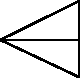
\includegraphics[scale=1]{gesamttex/edit_VIII-4/images/LH_35_13_03_220-221_d10_221v.pdf}
\edcaption{\lbrack\textit{Fig.~10}\rbrack}
\end{edfigure}
